\newcommand{\qe}[3]{\begin{quotation} \textit{``#1``} \end{quotation} \begin{flushright} - #2\end{flushright} }

\chapter{Forenzná analýza}


\qe{Aplikovanie metodickej sady techník a procedúr potrebných na získanie dôkazov z dodaného počítačového vybavenia, rôznych pamäťových zariadení a digitálnych médii, ktoré môžu byť následne prezentované v koherentnom a zmysluplnom formáte.}{Dr. H.B. Wolfe}

Incidenty v informačnej bezpečnosti sa odohrávajú vo virtuálnom priestore počítačov a počítačových sieti. V ideálnom prípade by sme mali byť schopní zabrániť prípadným útokom, no nie vždy je to možné. Ak už k bezpečnostnému incidentu dôjde, je potrebné zaistiť dôkazy, správne ich vyhodnotiť a na ich základe vyvodiť závery.

Forenzná analýza je jednou z používaných analýz pri vyšetrovaní trestných činov. Cieľom počítačovej forenznej analýzy je príprava získaných materiálov na ďalšie vyšetrovanie. Rieši problematiku kto, ako a kedy uskutočnil nejakú aktivitu súvisiacu s vykonaným trestným činom. Zahŕňa využitie širokého spektra vyšetrovacích technológií a postupov a metód. Slúži ako prostriedok na získanie dôkazov k trestným činom, zneužitie právomocí, porušenie zákona, interných pravidiel alebo smerníc, preukázanie identity osôb, pravosti listín, dát alebo informácií a to ako účastníkom trestného konania tak aj komerčnej sfére. Musí byť vykonávaná podľa prísnych pravidiel aby boli dôkazy prijateľné pre organy činne v trestnom konaní. Počas forenznej analýzy je kľúčové zbieranie digitálneho dôkazového materiálu. Predmetom skúmania nie sú často len samostatné počítače, ale celé počítačové systémy. Výsledkom forenznej analýzy je znalecký alebo technický posudok alebo vyjadrenie, ktorý má v súdnom konaní dôkazovú hodnotu.

\section{Mobilná forenzná analýza}

\qe{Mobilná forenzná analýza je veda zaoberajúca sa obnovou digitálnych dát z mobilných zariadení podľa striktných foreznych pravidiel za pomoci schválených metód.}{National Institute of Standards and Technology
(NIST)}

Získavanie digitálnych dokázov v mobilných forenzných aktivitách zahŕňa fyzické, logické,
a ručné metódy. Fyzické spôsoby získavania dôkazov sa týkajú obnovy binárne reprezentácie internej pamäte mobilných zariadení
a ich ukladania do súborov. Logické spôsoby pracujú s operačným systémom skúmaného mobilného zariadenia za účelom obnovy logických objektov v súborovom systéme. Ručné spôsoby zahŕňajú zobrazovanie dátového obsahu uloženého v mobilnom zariadení, ktoré vyžaduje manuálnu aktivitu s tlačidlami, klávesnicou či dotykovou obrazovkou a môžu byť nahrávané na externú digitálnu kameru. 

Existujúci výskum v oblasti mobilnej forenznej analýzy je možné klasifikovať do nasledovných častí: 1. preskúmanie možností metód získavania dôkazov, 2. vykonávanie podrobných forenzných postupov, 3. vykonávanie hĺbkovej forenznej analýzy mobilných aplikácií alebo mobilných operačných systémov. 

\begin{figure}[h]
	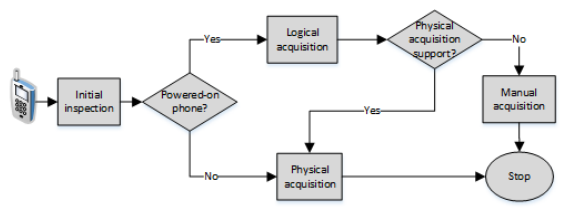
\includegraphics[width=\textwidth]{ziskavanie_dat}
	\caption{Procedúra získavania dát}
\end{figure}


Počiatočná kontrola predstavuje činnosť preskúmania stavu zariadenia zhromažďovaním informácií ako napríklad výrobcu zariadenia, názvu modelu a čísla IMEI. Stav zariadenia rozhoduje o použití techník na získavanie dôkazov. Logické získavanie dôkazov sa vykoná v prípade, že zariadenie je zapnuté. Začína identifikáciou zmeškaných hovorov, neprečítaných správ, času a dátumu pomocou skúmania obrazovky zariadenia. 

Fyzické získavanie dôkazov je vykonávané ak je zariadenie vypnuté. Vykonávanie ručného získavania dôkazov je voliteľné, ak výsledky z logického skúmania sú obmedzené a/alebo fyzické skúmanie nie je podporované. 

\chapter{Terorizmus a mobilné aplikácie}
Mobilné technológie sú často zneužívané na aktivity súvisiace s terorizmom. Forenzná analýza je dôležitý prostriedok pri vyšetrovaní takýchto aktivít. Terorizmus možno definovať ako použitie násilia skupinami alebo jednotlivcami, ktorí sa snažia presadiť svoje politické ciele. Svoje ciele si vyberajú náhodne, často ide o spôsobenie čo najväčších civilných strát.

V nedávnej dobe došlo k incidentu, kedy spoločnosť Apple Inc. odmietla pomôcť Federálnemu vyšetrovaciemu úradu v USA so žiadosťou o odblokovanie šifrovaného iPhone 5C údajne
patriacemu jednému z kľúčových podozrivých, pretože podozrivý deaktivoval iCloud zálohy niekoľko týždňov pred incidentom\footnote{\url{https://assets.documentcloud.org/documents/2716811/Statement-from-the-FBI-Feb-20-2016.pdf}}.

Tento incident si získal znateľný záujem medií, ako aj rozvíril debaty medzi v výskumníkmi a politikmi. Taktiež demonštroval potenciálnu úlohu mobilnej forenznej analýzy pri obnove dôkazových materiálov z mobilných zariadení, ktoré boli použité pri plánovaní, vykonávaní terorizmu a iných kriminálnych aktivít.

Cloudové aplikácie môžu byť používané na ukladanie dát, ktoré môže byť neskôr použité pri vyšetrovaní ako dôkazový materiál \cite{Cahyani:2016:RMF:3021385.3021421}.
Komunikačné aplikácie slúžia na výmenu hlasových a video správ. Môžu teda obsahovať potenciálne informácie o plánovaní a organizácie kriminálnych aktivít.
Pomocou forenzných techník je možné obnoviť záznamy z konverzácií, multimediálne súbory, zoznamy kontaktov, geografické dáta, ktoré sú neskôr použité na určenie sledu udalosti a identifikácie rôznych súvislostí týkajúcich sa trestného činu.

\chapter{Reverzné inžinierstvo v mobilnej forenznej analýze}

Získavanie dát z mobilných zariadení je zložité kvôli rôznych dôvodom \cite{Wilson:2017:CSM:3077286.3077564}. Pre obnovu dát je potrebné aby vyšetrovatelia najskôr získali uložené dáta za zariadenia. Samotné získavanie je ťažkopádne, ale
často ho možno dosiahnuť použitím špeciálnych nástrojov. Je užitočné, ale nie je dostatočné na získanie dát zo zariadenia iba pomocou rozhrania alebo softvéru mobilné zariadenia. Odstránené dáta nemôžu byť získané a vymazané informácie nemôžu byť obnovené. Navyše proces zobrazenia dát môže pozmeniť určité informácie (napr. zmena času posledného prístupu).

Po získaní dát je potrebné ich interpretovať a vytiahnuť z nich potrebné informácie.
Na druhej strane, softvér mobilného zariadenia je vo veľkej miere chránený a výrobcovia odmietajú pomáhať s cieľom chrániť si obchodné tajomstvá. V praxi je teda potrebné použiť reverzné inžinierstvo na preskúmanie formátu dát.

Cieľom reverzného inžinierstva je interpretovať dáta, ktoré boli vytvorené podľa neznámej formátovej špecifikácie S skúmaním reprezentatívnych vzoriek dát. Predpokladajme, že máme sadu vzoriek $R = \{r_{1}, r_{2}, ..., r_{n}\}$. Každá vzorka dát je vytvorená podľa $S$ a skladá z jedného alebo viacerých neprekrývajúcich sa polí. Platí, že $r_{i} = \{f_{1}, f_{2}, ..., f_{n}\}$. Pole predstavuje zmysluplný súbor údajov, napríklad celé číslo alebo reťazec. Predpokladáme, že hranice medzi políčkami nie sú známe a že v zázname nie sú žiadne explicitné oddeľovače polí. Inými slovami, bez znalosti formátu, každý záznam je to postupnosťou binárnych dát. Pre každý záznam $r_{i}$ je cieľom poskytnúť predpokladaný výklad $r^{'}_{i}$. Táto interpretácia zahŕňa východiskovú pozíciu $s$, dĺžku $l$, typ $t$ každého poľa v zázname tak, že $r^{'}_{i} = \{f^{'}_{1}, f^{'}_{2}, ..., f^{'}_{n}\}$, kde $f^{'}_{j}$ je trojica $(s_{j}, l_{j}, t_{j})$.

Niekoľko spoločností predávajú nástroje na analýzu dát v mobilných zariadeniach za pomoci znalostí získaných z manuálne ručného reverzného inžinierstva. Tento proces je náročný a musí sa často opakovať z dôvodu vývoja a predaja nových zariadení. V dôsledku toho tieto nástroje
môžu byť veľmi drahé - niektoré dosahujú cenu 20 000 dolárov. 

Avšak i celá sada týchto mnohých forenzných nástrojov nepokrýva veľkú množinu dostupných mobilných zariadení. Tieto dôvody iniciovali mnoho pokusov na uľahčenia procesu reverzného inžinierstva.

\section{Prístup založený na vzorkách}

Existuje viacero nástrojov, ktoré používajú techniku vzorkovania vstupných dát na vzorky za účelom odvodenia formátu dát.

Discoverer \cite{Cui:2007:DAP:1362903.1362917} sa snaží automaticky odvodiť formát správ zasielaných sieťovým protokolom na úrovni aplikačnej vrstvy. Po získaní vzorku, Discoverer rozdelí každú správu do tokenov, zhlukuje každý token a pokúša sa odvodiť formát tokenu porovnaním s iným správami v rovnakom zhluku.

LearnPADS \cite{Fisher:2008:DSF:1328897.1328488} je ďalší nástroj využívajúci vzorkovaní na odvodzovanie formátu ad hoc dát. Vytvára špecifikáciu tohto formátu v jazyku PADS na opis dát.  LearnPADS začína rozdelím vstupných dát na série zhlukov, typicky riadok po riadku alebo súbor za súborom. Zhluky sa ďalej rozdeľujú do tokenov pomocou lexikálneho analyzátora. LearnPADS používa histogram frekvencií tokenov na odvodenie štruktúry dát.

\section{Prístup založený na inštrumentácii}

Mnoho prístupov, zahŕňajúc Polyglot \cite{Caballero:2007:PAE:1315245.1315286}, Tupni \cite{Cui:2008:TAR:1455770.1455820} a Dispatcher \cite{Caballero:2009:DEA:1653662.1653737}, vyžaduje komplexný proces inštrumentácie binárneho spustiteľného súboru.

Polyglot bol vytvorený na prekonanie nedostatkov prístupov založených na vzorkách
sledovaním toho, ako program spracováva prijaté správy. Tupni používa tzv. taint analýzu na spätné vytváranie vstupných formátov s vysokou presnosťou. Dispatcher sa taktiež snaží odvodiť formát správ odoslaných programom, ako aj sémantiku polí v odosielaných a prijatých správach.

\chapter{Forenzná analýza prevádzky mobilných zariadení}

Telefónne spoločnosti musia podľa súčasné predpisy mať záznamy týkajúce sa prevádzky telefónov za dané časové obdobie \cite{Catanese:2010:VTF:1877972.1877992}. Tieto súbory obsahujú obrovské množstvo dát, ako sú telefonické hovory, SMS, MMS, GPRS a internetové služby. Zaujímavé informácie sú tiež získané z prevádzky, ktorú produkuje bunka Global Identities (CGI) vo vnútri týchto oblastiach. Analýza správ od telefónnych spoločností umožňuje rekonštrukciu vzťahov medzi jednotlivcami v sieti

Vzťahy vytvorené prostredníctvom telefonickej prevádzky možno preskúmať prostredníctvom rôznych techník. Niektoré forenzné analýzy sa týka telefónnej prevádzky uskutočnenej pomocou International Mobile Subscriber Identity (IMSI) a International Mobile Equipment Identity (IMEI). IMSI je jedinečné číslo spojené so všetkými GSM a UMTS užívateľmi. Je uložené na SIM karte
v telefóne a je odosielané telefónom do siete. IMEI je jedinečný 15 alebo 17-miestny kód používaný na identifikáciu mobilnej stanice v sieti GSM alebo UMTS. 

Detektívi vo všeobecnosti rozlišujú tri hlavné typy analýzy denníka prevádzky telefónu. Prvá skúma vzťahy medzi individuálnymi užívateľmi. Druhá sa zaoberá geografickou polohou telefónu a tretia skúma udalosti v prevádzke v časovej ose.

\newpage

\section{Analýza záznamov -- LogAnalysis}
\it{LogAnalysis} sa zaoberá na prvý typom analýzy denníka telefónu.

\begin{figure}[h]
	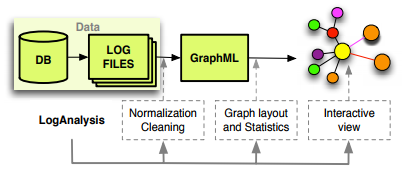
\includegraphics[width=\textwidth]{log_analyza}
	\caption{Architektúra \it{LogAnalysis}}
\end{figure}

Architektúra je tvorená rozšíriteľnými úrovňami: import dát vytvorenými informatívnymi
systémami mobilných telefónov (zvyčajne bytové súbory), konverzie do formátu GraphML, ktorý je štruktúrovaný formát XML vhodnejší pre grafické znázornenie a výmeny medzi aplikáciami na kreslenie grafov.

Cieľom je získať zaujímavé informácie pre vyšetrovanie z celkovej štruktúry siete.
